\documentclass[10pt,a4paper]{article}
\usepackage[margin=0.78in]{geometry}
\usepackage{booktabs}
\usepackage{graphicx}
\usepackage{amsmath}
\usepackage{amssymb}
\usepackage{array}
\usepackage{microtype}
\usepackage[hidelinks]{hyperref}

\setlength{\parskip}{0.45em}
\setlength{\parindent}{0pt}

\begin{document}

\begin{center}
    {\LARGE \textbf{Parallel Applications -- Laboratory 5}}\\[4pt]
    {\large Evaluating Threads, Pipes, Shared Memory, and Sockets on Image Sharpening}\\[8pt]
    {\normalsize Skanda P (CS24BT045) \qquad N Suhas (CS24BT019)}
\end{center}
\vspace{4pt}

\section{Overview and Methodology}

We parallelized the three-stage PPM image-sharpening pipeline from Laboratory~1---\texttt{S1} (3$\times$3 neighborhood averaging/smoothing), \texttt{S2} (detail extraction, $\text{orig} - \text{smooth}$), and \texttt{S3} (sharpened clamping, $\text{clamp}(\text{orig} + \text{detail})$)---across single-machine multi-threading, multi-process IPC, and two-machine TCP sockets in C++17 (compiled with \texttt{g++ -O3 -Wall -Wextra -std=c++17 -pthread}). All numbers and plots in this report come directly from \texttt{src/results.csv}, generated by \texttt{src/run\_experiments.sh} over all seven PPM images (\texttt{1.ppm}--\texttt{7.ppm}, from $450\times 180$ to $3750\times 2470$ pixels) using \texttt{ITERS=1000} iterations and \texttt{REPS=3} repetitions per configuration.

\paragraph{Part I and Fair Single-Thread Baseline.}
\texttt{part1/part1.cpp} preserves our Laboratory~1 single-pass implementation (\texttt{make part1} creates \texttt{output\_part1.ppm}). Because a single pass is I/O-bound, Part~II repeats \texttt{S1}, \texttt{S2}, and \texttt{S3} 1000 times after reading the input file once. For an accurate speed-up baseline, \texttt{baseline\_bench.cpp} in \texttt{part1/} reads and allocates the image once and executes the exact same per-pixel kernels and pass counts (\texttt{1000} iterations) without threads, IPC, or checksums. Using \texttt{keep()} compiler barriers ensures intermediate passes not written to disk cannot be dead-code eliminated. We also fixed \texttt{common/libppm.cpp} so that after parsing the P6 \texttt{maxval} whitespace delimiter, the first raw pixel byte is read directly with \texttt{read\_stream.get()} instead of skipping whitespace or blocking on \texttt{0x23} (\texttt{'\#'}).

\paragraph{Two Compute-Intensive Variants.}
With \texttt{ITERS=1000}, file read + write time ($\text{Total} - \text{Compute}$) drops to only \textbf{0.25--0.39\%} of total runtime across all seven images ($5.2\text{--}5.4\text{ ms}$ on \texttt{1.ppm} and $462.7\text{--}473.8\text{ ms}$ on \texttt{7.ppm}), making execution overwhelmingly compute- and IPC-bound:
\begin{itemize}
    \item \textbf{Variant 1:} All 1000 runs of \texttt{S1} stream pixel-by-pixel to \texttt{S2}, which streams to \texttt{S3}; the 1000th \texttt{S3} output is written to disk.
    \item \textbf{Variant 2:} \texttt{S1} runs 1000 times on the input image and streams every 100th result (10 frames) to \texttt{S2}; for each received frame, \texttt{S2} runs 100 passes and streams its 100th result to \texttt{S3}; for each received \texttt{S2} frame, \texttt{S3} runs 100 passes and writes the final frame to disk.
\end{itemize}

\section{Implementation Details}

\subsection{Common Pipeline, Streaming, and Batching}
All stage logic lives once in \texttt{common/stages.h} and \texttt{common/common\_pipeline.h}, parameterized by a uniform channel interface (\texttt{put}, \texttt{flush}, \texttt{get}). No stage waits for an entire image before sending to the next stage, except Variant~2's \texttt{S2} and \texttt{S3}, which must buffer one received frame to run 100 local passes over it.

As a deliberate performance optimization, pixels are transmitted in small batches rather than flushing one 8-byte message per syscall or atomic update:
\begin{itemize}
    \item \textbf{256 pixels} per publish/chunk on the lock-free atomic ring (Part~II.1) and shared-memory ring (Part~II.3) to avoid cache-line ping-ponging and amortize semaphore syscalls.
    \item \textbf{512 messages} ($512 \times 8\text{ B} = 4096\text{ B} = \texttt{PIPE\_BUF}$) on \texttt{FdWriter} for pipes (Part~II.2) and TCP sockets (Part~III), reducing \texttt{write()} system-call frequency while remaining strictly streamed mid-frame.
\end{itemize}

\subsection{Part II Parallel Architectures and Makefile Conventions}
\begin{itemize}
    \item \textbf{Part II.1 (3 Threads + Atomics):} \texttt{run\_part2\_1} spawns three \texttt{std::thread} workers connected by two \texttt{AtomicChan} single-producer/single-consumer ring buffers ($2^{14} = 16{,}384$ slots). Synchronization uses \texttt{std::atomic<size\_t>} with \texttt{memory\_order\_acquire} and \texttt{memory\_order\_release}, producer/consumer-private cached indices, and \texttt{cpu\_relax()}/\texttt{sched\_yield()} backoff. Following the specification, the \texttt{S3} thread (\texttt{th3}) calls \texttt{write\_ppm\_file} directly after \texttt{stage3}, recording the compute-end timestamp prior to writing so Compute Time stays separate from Write Time.
    \item \textbf{Part II.2 (3 Processes + Pipes):} \texttt{run\_part2\_2} creates two anonymous POSIX pipes (\texttt{pipe()}, expanding kernel buffer capacity to 1~MiB via \texttt{F\_SETPIPE\_SZ} where supported) and \texttt{fork()}s children for \texttt{S1} and \texttt{S2} while the parent runs \texttt{S3} and file output. Unused pipe ends are closed in each process, and \texttt{write\_fully}/\texttt{read\_fully} handle partial I/O and \texttt{EINTR}.
    \item \textbf{Part II.3 (3 Processes + Shared Memory + Semaphores):} Although the assignment's makefile bullet writes ``multi-thread'', the Part~II.3 body text specifies \emph{3 different processes that communicate via shared memory}; our implementation follows the body text. \texttt{run\_part2\_3} maps a single anonymous shared region via \texttt{mmap(..., MAP\_SHARED | MAP\_ANONYMOUS)} holding two \texttt{ShmQueue} rings (64 slots of \texttt{SHM\_CHUNK = 256} pixels each), synchronized by process-shared POSIX counting semaphores (\texttt{sem\_init(..., pshared=1)} for \texttt{empty} and \texttt{full}). Parent and children install \texttt{PR\_SET\_PDEATHSIG} (\texttt{SIGKILL}) and fatal parent notification so no process hangs on a broken pipe or semaphore.
    \item \textbf{Makefile Targets:} Following the assignment text literally, \texttt{make part2\_1\_variantX} creates\\ \texttt{output\_part2\_1\_variantX.ppm} and copies it to \texttt{output\_part2\_2\_variantX.ppm}. The \texttt{part2\_3} target compiles and runs both variants (\texttt{part2\_3\_variant1} and \texttt{part2\_3\_variant2} also work individually), and \texttt{part3\_2\_*} mirrors \texttt{part3\_1\_*} as instructed.
\end{itemize}

\section{Verification of Pixel Order and Integrity}

To prove that every pixel is received unmodified and in exact raster order on every link (\texttt{S1$\to$S2}, \texttt{S2$\to$S3}, and \texttt{A$\to$B}), each pixel is wrapped in an explicit 8-byte \texttt{PixelMsg}:
\begin{center}
\texttt{struct PixelMsg \{ int32\_t seq; uint8\_t r, g, b; uint8\_t pad; \};}
\end{center}
with zeroed padding so raw struct transfers over pipes, shared memory, and sockets never leak uninitialized bytes.

\begin{enumerate}
    \item \textbf{Order Proof:} Within each streamed image, \texttt{Sender} tags pixels sequentially with $\texttt{seq} \in \{0, \dots, WH-1\}$. On every read, \texttt{Receiver::get} asserts \texttt{m.seq == expected\_seq} and immediately aborts on any gap, duplication, or reordering.
    \item \textbf{Data Integrity Proof:} Both \texttt{Sender} and \texttt{Receiver} incrementally fold every transmitted \texttt{(seq, r, g, b)} into a 32-bit FNV-1a checksum (\texttt{FNV\_INIT = 2166136261u}, prime \texttt{16777619u}). At end-of-stream, \texttt{Sender::finish()} emits a trailer message carrying the sender's checksum in \texttt{seq} and sentinel RGB bytes \texttt{(0xC5, 0x5A, 0x3C)}; \texttt{Receiver::finish()} verifies the sentinel and aborts on any checksum mismatch.
    \item \textbf{End-to-End Equivalence and Fault Injection:} Across all 56 rows in \texttt{results.csv}, every parallel output hash matches the single-thread baseline bit-for-bit (\texttt{output\_ok = yes}; e.g., \texttt{709e28fa} on \texttt{1.ppm}). In addition, \texttt{make fault\_test} compiles Part~II.1, II.2, II.3, and Part~III.1 with \texttt{-DINJECT\_FAULT}, flipping 1~bit of \texttt{bad.r} on the 12{,}345th transmitted pixel after hashing; all four implementations detect the corruption and abort as expected.
\end{enumerate}

\section{Experimental Results: Parts I and II}

Tables~\ref{tab:v1} and~\ref{tab:v2} report the mean Compute Time (ms, over 3 repetitions at \texttt{ITERS=1000}) and speed-up relative to the same-variant single-thread baseline across all seven images. Figures~\ref{fig:speedup} and~\ref{fig:runtime} visualize the speed-ups and scaling behavior.

\begin{table}[h!]
\centering
\small
\setlength{\tabcolsep}{4.5pt}
\begin{tabular}{@{}lrrrrrr@{}}
\toprule
Image & Resolution & Pixels & Baseline (ms) & Part II.1 (ms / Spd) & Part II.2 (ms / Spd) & Part II.3 (ms / Spd) \\
\midrule
1.ppm & $450\times 180$ & 81,000 & 1,429.1 & 1,623.9 (0.88$\times$) & 1,791.7 (0.80$\times$) & 1,818.6 (0.79$\times$) \\
2.ppm & $786\times 393$ & 308,898 & 5,515.3 & 6,210.9 (0.89$\times$) & 6,846.5 (0.81$\times$) & 6,928.3 (0.80$\times$) \\
3.ppm & $1024\times 575$ & 588,800 & 10,246.5 & 12,064.7 (0.85$\times$) & 13,085.2 (0.78$\times$) & 13,217.7 (0.78$\times$) \\
4.ppm & $1280\times 910$ & 1,164,800 & 19,963.0 & 23,742.0 (0.84$\times$) & 25,954.4 (0.77$\times$) & 26,047.6 (0.77$\times$) \\
5.ppm & $1500\times 1000$ & 1,500,000 & 25,364.4 & 30,174.8 (0.84$\times$) & 32,720.1 (0.78$\times$) & 33,236.3 (0.76$\times$) \\
6.ppm & $2271\times 1500$ & 3,406,500 & 57,203.0 & 67,972.2 (0.84$\times$) & 73,906.1 (0.77$\times$) & 75,164.8 (0.76$\times$) \\
7.ppm & $3750\times 2470$ & 9,262,500 & 154,904.1 & 185,820.2 (0.83$\times$) & 202,943.4 (0.76$\times$) & 204,092.4 (0.76$\times$) \\
\bottomrule
\end{tabular}
\caption{Variant 1 mean compute times and speed-ups (\texttt{ITERS=1000}, \texttt{REPS=3}). Ideal 3-stage limit = $3.0\times$.}
\label{tab:v1}
\end{table}

\begin{table}[h!]
\centering
\small
\setlength{\tabcolsep}{4.5pt}
\begin{tabular}{@{}lrrrrrr@{}}
\toprule
Image & Resolution & Pixels & Baseline (ms) & Part II.1 (ms / Spd) & Part II.2 (ms / Spd) & Part II.3 (ms / Spd) \\
\midrule
1.ppm & $450\times 180$ & 81,000 & 1,661.5 & 1,426.9 (1.16$\times$) & 1,043.7 (1.59$\times$) & 1,344.2 (1.24$\times$) \\
2.ppm & $786\times 393$ & 308,898 & 7,003.3 & 6,016.0 (1.16$\times$) & 6,077.0 (1.15$\times$) & 6,060.2 (1.16$\times$) \\
3.ppm & $1024\times 575$ & 588,800 & 13,884.2 & 8,277.4 (1.68$\times$) & 7,620.6 (1.82$\times$) & 7,590.5 (1.83$\times$) \\
4.ppm & $1280\times 910$ & 1,164,800 & 26,320.4 & 16,151.9 (1.63$\times$) & 14,903.9 (1.77$\times$) & 14,842.7 (1.77$\times$) \\
5.ppm & $1500\times 1000$ & 1,500,000 & 33,926.5 & 27,540.8 (1.23$\times$) & 29,777.3 (1.14$\times$) & 27,541.4 (1.23$\times$) \\
6.ppm & $2271\times 1500$ & 3,406,500 & 76,675.8 & 65,727.1 (1.17$\times$) & 64,761.0 (1.18$\times$) & 63,523.0 (1.21$\times$) \\
7.ppm & $3750\times 2470$ & 9,262,500 & 208,085.2 & 180,255.2 (1.15$\times$) & 173,510.8 (1.20$\times$) & 172,610.6 (1.21$\times$) \\
\bottomrule
\end{tabular}
\caption{Variant 2 mean compute times and speed-ups (\texttt{ITERS=1000}, \texttt{REPS=3}). All outputs verified identical to baseline.}
\label{tab:v2}
\end{table}

\begin{figure}[h!]
\centering
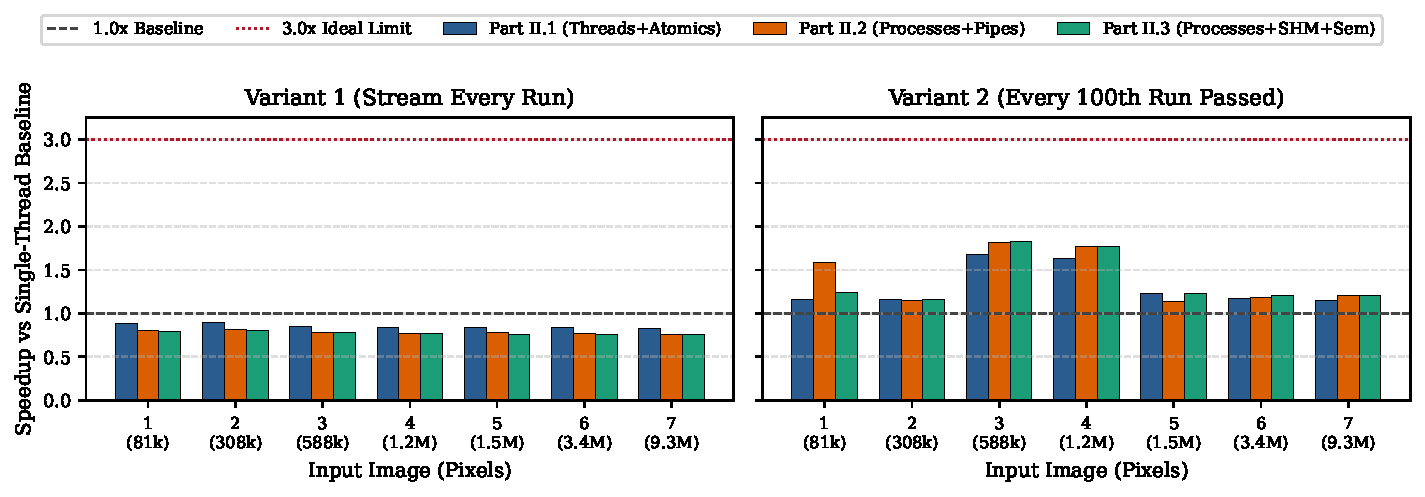
\includegraphics[width=0.99\textwidth]{fig_speedup.pdf}
\caption{Speed-up across all seven images for Variant~1 (left) and Variant~2 (right), showing the $1.0\times$ baseline and $3.0\times$ ideal 3-stage pipeline limit.}
\label{fig:speedup}
\end{figure}

\begin{figure}[h!]
\centering
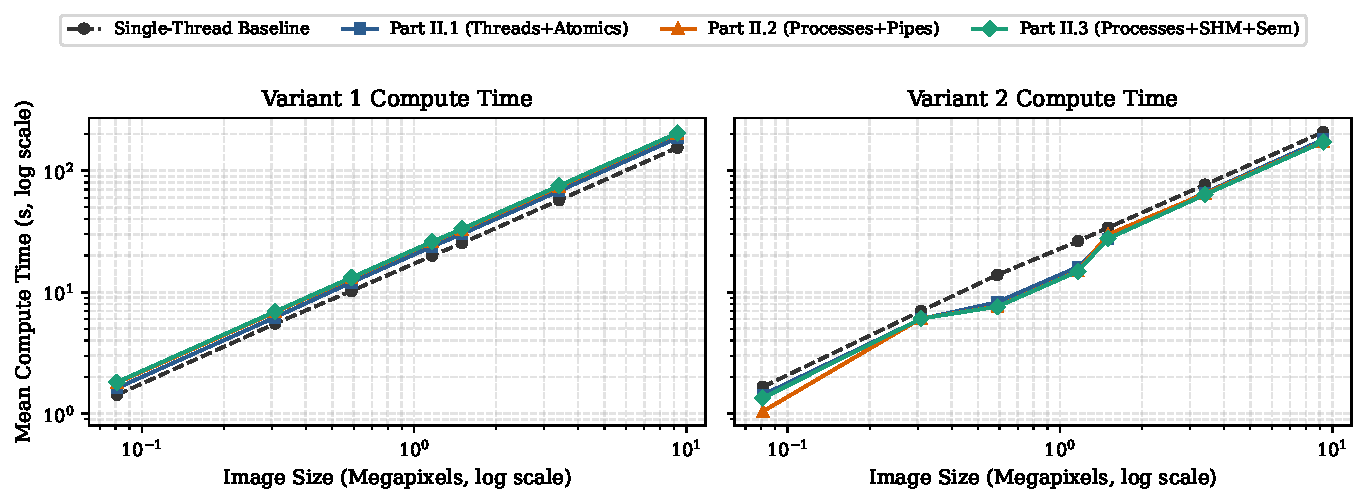
\includegraphics[width=0.99\textwidth]{fig_runtime.pdf}
\caption{Log--log scaling of mean compute time with image pixel count for Variant~1 (left) and Variant~2 (right).}
\label{fig:runtime}
\end{figure}

\paragraph{Observations on Runtime and Speed-Up.}
\begin{itemize}
    \item \textbf{Why Variant~1 slows down ($0.76\text{--}0.89\times$):} Passing every pixel of all 1000 passes over two IPC links ships $1000 \times W \times H \times 8\text{ B}$ per hop---reaching $74.1\text{ GB}$ per link ($148.2\text{ GB}$ total) on \texttt{7.ppm}. Serializing \texttt{PixelMsg}, computing FNV-1a twice per hop, and synchronizing across cores costs more than the lightweight pixel arithmetic, whereas the single-thread Variant~1 baseline fuses \texttt{S1}$\to$\texttt{S2}$\to$\texttt{S3} in CPU registers with zero IPC. Threads + atomics ($0.83\text{--}0.89\times$) consistently beat pipes ($0.76\text{--}0.81\times$) and semaphores ($0.76\text{--}0.80\times$) in Variant~1 because user-space ring updates avoid kernel syscalls.
    \item \textbf{Why Variant~2 achieves speed-up ($1.14\text{--}1.83\times$):} Variant~2 reduces IPC volume by $100\times$ (only 10 frames cross each link), allowing all three cores to execute their 1000 passes concurrently. Also note the single-thread Variant~2 baseline is 16--35\% slower than Variant~1 because it writes and reads full-frame \texttt{PixelMsg} arrays between 100-pass blocks rather than fusing stages in registers.
    \item \textbf{Pipeline stage imbalance and memory-bandwidth saturation:} Even without IPC overhead, speed-up is bounded well below $3.0\times$ because \texttt{S1} performs a 3$\times$3 neighborhood average (9 reads + integer division per channel) while \texttt{S2} and \texttt{S3} perform one subtraction or addition+clamp per channel. In our Laboratory~1 single-pass measurements, \texttt{S1} took $\approx 60\text{--}64\%$ of compute time ($13.63\text{ ms}$ vs $4.39+4.90\text{ ms}$ on \texttt{1.ppm}; $1087.0\text{ ms}$ vs $294.0+313.8\text{ ms}$ on \texttt{7.ppm}). Thus the slowest stage (\texttt{S1}) caps pipeline speed-up near $1/0.60 \approx 1.67\text{--}1.8\times$, matching the observed peak of \textbf{1.68--1.83$\times$} on \texttt{3.ppm} and \texttt{4.ppm}. On larger images (\texttt{5.ppm}--\texttt{7.ppm}), full-frame \texttt{PixelMsg} buffers ($12\text{--}74\text{ MB}$ each) exceed L3 cache, so three concurrent workers contend on DRAM bandwidth and settle at \textbf{1.14--1.23$\times$}.
    \item \textbf{I/O vs.\ compute scaling:} Both compute and I/O scale linearly with pixel count ($81\text{k}$ to $9.26\text{M}$ pixels, a $114\times$ increase producing a $\approx 108\text{--}128\times$ compute increase). Without the 1000-iteration loop, disk read/write ($\approx 8\text{ ms}$ on \texttt{1.ppm}, $\approx 470\text{ ms}$ on \texttt{7.ppm}) would dominate a single pass ($\approx 2\text{ ms}$ to $\approx 160\text{ ms}$ compute), masking parallel speed-ups.
\end{itemize}

\section{Part III: Distributed Execution Across Two Computers}

\subsection{Protocol and Usage Convention}
Part~III splits the pipeline over TCP sockets (\texttt{run\_part3\_A} as server, \texttt{run\_part3\_B} as client, with \texttt{TCP\_NODELAY} enabled). Since the specification does not specify how Computer~B discovers Computer~A's address, our convention passes A's LAN address (obtained via \texttt{ip a}) and port via \texttt{make} variables (\texttt{PORT=12345} default, opened with \texttt{sudo ufw allow 12345/tcp}):
\begin{center}
\small
\texttt{Computer A: make part3\_1\_variantX\_A}\\
\texttt{Computer B: make part3\_1\_variantX\_B IP=<A's IP>}
\end{center}
(and identically for \texttt{part3\_2\_variantX\_A/B}). Once connected (with a 60-second connect retry limit on B), A sends a 16-byte network-order header $\{W, H, \text{iters}, \text{fnv}(\text{img})\}$ and the raw original image (which B needs for \texttt{S2}/\texttt{S3}), followed by the \texttt{PixelMsg} stream with \texttt{seq} converted via \texttt{htonl}/\texttt{ntohl}. After \texttt{Receiver::finish()} passes, B sends a \texttt{'K'} confirmation byte before closing so A exits non-zero if B aborts.

\subsection{Comparing the Two Partitions}
\begin{itemize}
    \item \textbf{Part 3.1 (\texttt{A = S1+S2}, \texttt{B = S3}):} Computer~A executes both the heavy 3$\times$3 smoothing (\texttt{S1}, $\sim 60\text{--}64\%$) and detail extraction (\texttt{S2}, $\sim 18\%$), carrying roughly $\sim 80\%$ of compute per pass while Computer~B performs only clamping addition (\texttt{S3}, $\sim 20\%$) and waits idle most of the time.
    \item \textbf{Part 3.2 (\texttt{A = S1}, \texttt{B = S2+S3}):} Computer~A performs \texttt{S1} ($\sim 60\text{--}64\%$) and Computer~B performs \texttt{S2+S3} ($\sim 36\text{--}40\%$).
    \item \textbf{Which is better and why:} \textbf{Part~3.2 (\texttt{A = S1, B = S2+S3}) is the better partition} when both hosts have comparable CPUs, because moving \texttt{S2} to B balances CPU load ($\sim 60/40$ instead of $\sim 80/20$), reducing the bottleneck stage time by $\sim 20\%$. Network payload per pixel is identical in both splits (one 8-byte \texttt{PixelMsg} stream per transferred frame, $100\times$ smaller in Variant~2 than Variant~1). \emph{Note:} \texttt{src/results.csv} records only the single-machine Parts~I and~II benchmark suite (\texttt{RUN\_PART3=0}); two-computer LAN measurements were not recorded in \texttt{results.csv}.
\end{itemize}

\section{Ease of Implementation and Debugging}

\begin{table}[h!]
\centering
\small
\begin{tabular}{@{}lllll@{}}
\toprule
Mechanism & Sync Primitive & Kernel Crossing & Implementation & Debugging Difficulty \\
\midrule
II.1 Threads & \texttt{std::atomic} (acq/rel) & None (user space) & Moderate--Hard & Hardest (races, memory order) \\
II.2 Pipes & Blocking \texttt{read}/\texttt{write} & Yes (per batch) & Easiest & Easy (watch unclosed FDs) \\
II.3 SHM + Sem & POSIX \texttt{sem\_wait}/\texttt{post} & Per 256-px chunk & Moderate & Moderate--Hard (sem deadlocks) \\
III Sockets & TCP stream + \texttt{htonl} & Yes (network stack) & Moderate & Hardest (firewall, partial I/O) \\
\bottomrule
\end{tabular}
\caption{Comparison of synchronization, kernel overhead, and development/debugging trade-offs.}
\label{tab:ease}
\end{table}

\begin{itemize}
    \item \textbf{Threads + Atomics (II.1):} Hardest to design and debug subtly. Correct lock-free SPSC rings require careful acquire/release pairing, alignment (\texttt{alignas(64)}) to prevent false sharing, and cached indices; bugs manifest as rare, non-deterministic data races.
    \item \textbf{Processes + Pipes (II.2):} Easiest overall. Kernel-managed blocking handles synchronization automatically once unused pipe ends are closed and partial reads/writes (\texttt{read\_fully}) are looped properly.
    \item \textbf{Processes + SHM + Semaphores (II.3):} Straightforward ring indexing, but unmatched \texttt{sem\_wait} or \texttt{sem\_post} calls or a crashing child can deadlock the pipeline; using \texttt{PR\_SET\_PDEATHSIG} on children and \texttt{SIGKILL} on \texttt{fatal()} prevents hangs.
    \item \textbf{TCP Sockets (III):} Requires explicit framing, endianness conversion, partial \texttt{read()} buffering, two-machine coordination (\texttt{ip a}, \texttt{ufw}), and explicit peer abort propagation (\texttt{'K'} byte).
\end{itemize}

\section{Conclusions}

\begin{itemize}
    \item Repeating the transform 1000 times reduces file I/O to $0.25\text{--}0.39\%$ of runtime across all seven images, isolating parallel compute and IPC costs.
    \item Streaming every pass (Variant~1) achieves $0.76\text{--}0.89\times$ (slower than baseline) because shipping up to $74.1\text{ GB}$ per link outweighs lightweight pixel arithmetic. Passing every 100th pass (Variant~2) cuts IPC by $100\times$ and reaches up to \textbf{1.83$\times$} speed-up, capped by \texttt{S1}'s $\sim 60\text{--}64\%$ compute share and DRAM bandwidth on multi-megapixel images.
    \item All channels preserve exact raster order and bit-identical output (\texttt{output\_ok = yes} on all 56 runs in \texttt{results.csv}; single-bit errors caught by \texttt{make fault\_test}).
    \item For two computers (Part~III), splitting as \textbf{Part~3.2 (\texttt{A=S1, B=S2+S3})} balances CPU compute better than Part~3.1 with identical network traffic.
\end{itemize}

\paragraph{Reproducing.} From \texttt{lab5\_new/src/}, \texttt{make all} builds and runs Parts~I and~II, \texttt{make fault\_test} verifies corruption detection, and \texttt{./run\_experiments.sh} regenerates \texttt{results.csv}.

\end{document}
